\chapter{Generaci\'on de configuraciones}\label{anexo-configuraciones}



\section{Configuraciones red polim\'erica nanogel}

La red de pol\'imeros que forma el nanogel tiene una topolog\'ia similar a la del diamante, donde los entrecruzamientos se colocan en la posici\'on original de los \'atomos de carbono y se conectan a cuatro cadenas de pol\'imeros.

Para construir esta red, primero definimos una estructura tridimensional donde todas las cadenas de pol\'imeros se alargan. Luego, solo conservamos aquellos segmentos contenidos dentro de una esfera de radio $R_{cut}$ colocada en el centro de masa de la estructura. $R_{cut}$ se elige de manera que la red resultante tenga aproximadamente $10^4$ segmentos. En total, la red que resulta de esta estrategia tiene 10026 segmentos.

\begin{figure}[!ht]
	\centering
	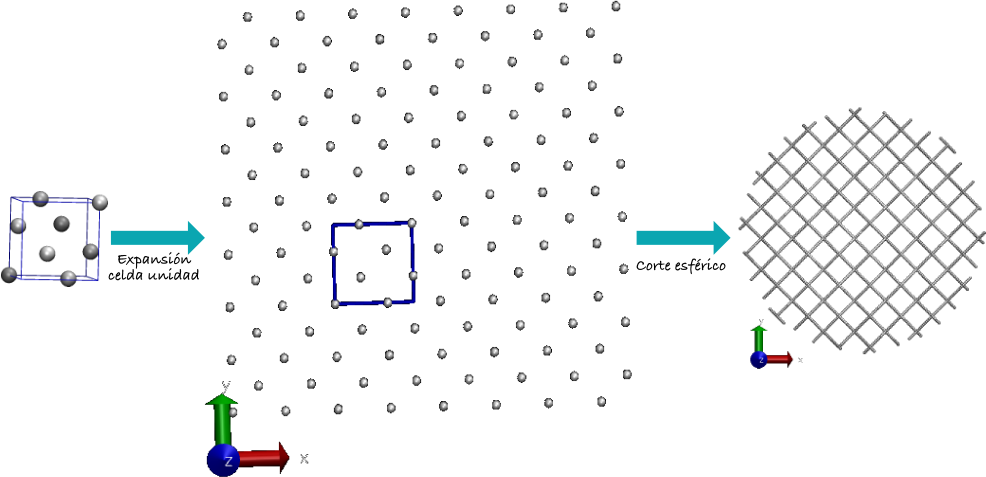
\includegraphics[width=0.5\linewidth]{Figures/graph-anexos/esquema.png}
	\caption{Estrucutra base para la generaci\'on de configuraciones de nanogeles}
	\label{fig:anexo:equema-gel}
\end{figure}




Originalmente, todas las cadenas de pol\'imeros conectan dos entrecruzamientos, pero como resultado del procedimiento mencionado anteriormente, algunas quedan colgando en la superficie de la red y se conectan solo a un entrecruzamiento. Estas cadenas colgantes contienen el 22\% del n\'umero total de segmentos.

Para obtener configuraciones de esta estructura, hemos realizado simulaciones de Din\'amica Molecular utilizando GROMACS 5.1.2 \cite{lindahl2001gromacs}
Para describir las interacciones no enlazadas entre los segmentos de la red, utilizamos un potencial de Leonard-Jones puramente repulsivo con un desplazamiento.

\begin{equation}
	V_{LJ}=\begin{cases}
		4\epsilon \left[\left(\frac{\sigma}{r_{ij}}\right)^{12} - \left(\frac{\sigma}{r_{ij}}\right)^{6}\right] + \epsilon & \text{if $r_{ij} < 2^{1/6}\sigma$}\\
		0 & \text{otro}.
	\end{cases}
\end{equation}



Donde $\epsilon = 1 k_BT$ y $\sigma = $ 0.5 nm, y $r_{ij}$ es la distancia entre los segmentos $i$ y $j$.
Para generar una variedad de configuraciones compactas de la estructura polim\'erica, en algunas simulaciones tambi\'en aplicamos una restricci\'on de posici\'on radial.
Este potencial se utiliza para restringir part\'iculas (en nuestro caso, los segmentos entrecruzadores de la red) a una regi\'on esf\'erica espec\'ifica del volumen de simulaci\'on.
Esta regi\'on esf\'erica esta delimitada por un radio $r_{fb}$.
De manera simplificada, la energ\'ia potencial asociada con esta fuerza externa tiene la siguiente forma:

\begin{equation}
	V_{fb}(r_i)=\begin{cases}
		0 & \text{if $r_{i} < r_{fb}$}\\
		\frac{1}{2}k_{fb}\left(r_i -r_{fb}\right)^2 & \text{otro}.
	\end{cases}
\end{equation}


Donde $r_i$ es la distancia entre la posici\'on del segmento entrecruzador $i$ y el centro de masa de la red, y $k_{fb}$ es la constante de fuerza.

Un enfoque similar puede utilizarse para generar conformaciones de red elongadas (hinchadas). En este caso, aplicamos un potencial arm\'onico que restringe las part\'iculas fuera de una regi\'on esférica espec\'ifica. Esta situaci\'on se describe utilizando valores negativos de $r_{fb}$, y este potencial solo se aplica a los entrecruzamientos m\'as superficiales de la red. M\'as detalles sobre estos potenciales con fondo plano se pueden encontrar en la referencia \cite{GROMACSRestraints}.

Para generar conformaciones compactas, hemos realizado simulaciones de Din\'amica Molecular utilizando $r_{fb} =$ 17.5, 20, 22.5 y 25 en unidades de $\sigma$.

Para conformaciones hinchadas, hemos utilizado valores de $r_{fb}$ desde $-80\sigma$ hasta $-50\sigma$ con un paso de $5\sigma$; y luego desde $-50\sigma$ hasta -27.5$\sigma$ con un paso de 2.5$\sigma$. Estos valores se refieren a la red libre (sin la restricci\'on potencial) que tiene un radio aproximado de $26\sigma$.
Se ha utilizado $k_{fb} = 50\frac{\varepsilon}{\sigma^2} $.



\begin{figure}[!ht]
	\centering
	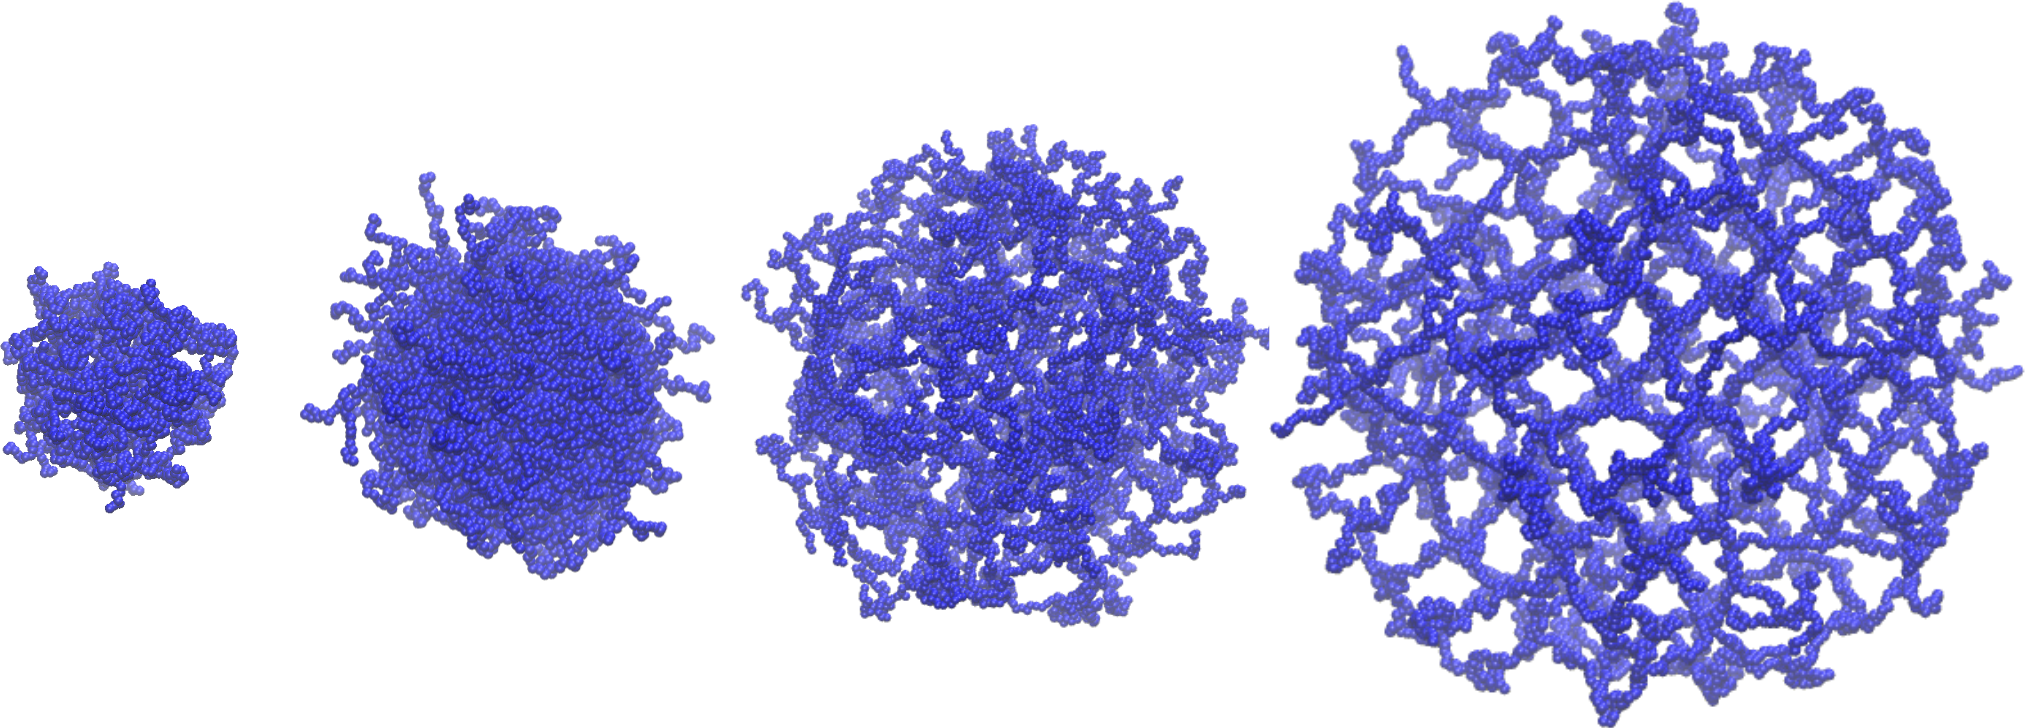
\includegraphics[width=0.5\linewidth]{Figures/graph-anexos/geles_radios.png}
	\caption{Direferentes radios originados con el potencial armonico de retricción. }
	\label{fig:anexo:geles}
\end{figure}


%Nuevamente, enfatizamos que, para obtener conformaciones m\'as compactas de la red polim\'erica, aplicamos el potencial con fondo plano a todos los entrecruzamientos de la red, mientras que para las conformaciones elongadas, la restricci\'on solo se aplica a los entrecruzamientos m\'as superficiales.

En cada ejecuci\'on de la simulaci\'on, el sistema se equilibr\'o durante 5 ns y luego la simulaci\'on continu\'o durante otros 10 ns. Durante este tiempo de producci\'on, se registr\'o una configuraci\'on cada 20 ps, lo que resulta en un total de 500 configuraciones por simulaci\'on y un total de 10000 configuraciones.
